
\section{Methods}

The development of the fully featured COMBINE archive can be divided into three major parts.
I first decided for a simulation study to encode in an archive, then I created an initial archive which was finally enriched with information I found on the internet and data that I generated on my own.
These steps are described in the following.

\subsection{Deciding for a Simulation Study}

I developed 3 criteria to decide for a simulation study:

\paragraph{Criteria 1: Open Access.}
As I want to share the demo archive openly, I need to find an experiment that offers as much open data as possible.
Obviously and unfortunately, the publication, which is an essential document for the documentation of experiments, is the bottleneck.
Therefore, I have to find a simulation experiment which was published using an open access license.

\paragraph{Criteria 2: Much data already available in standard formats.}
As I do not want to encoded the model myself, I only consider studies which are already available as SBML and CellML models.
Ideally, these models are already curated, which increases my trust in the encoding.

\paragraph{Criteria 3: I have ideally already dealt with that publication.}
As I will need to work with the study I need to understand it.
It usually takes a lot of time to dig into a new field, so I prefer studies that I already investigated.
However, this is just a soft criteria to decrease my workload.


\paragraph{Searching for a matching study.}
Searching for a study was harder than I thought.
I failed to encoded my search criteria in a format consumable by the search engines of current databases.
I ended up asking a common search engine to look for names of open access journals at the websites of the databases and eventually \texttt{site:models.cellml.org "Molecular Systems Biology"}\footnote{\href{https://duckduckgo.com/?q=site\%3Amodels.cellml.org+\%22Molecular+Systems+Biology\%22}{duckduckgo.com/?q=site\%3Amodels.cellml.org+\%22Molecular+Systems+Biology\%22}} resulted in a model that is available from the CellML model repository (Calzone, Thieffry, Tyson, Novak, 2007\footnote{\href{http://models.cellml.org/exposure/1a3f36d015121d5596565fe7d9afb332}{models.cellml.org/exposure/1a3f36d015121d5596565fe7d9afb332}})~\cite{cellmlrepo} and from the Biomodels Database (BIOMD0000000144\footnote{\href{http://www.ebi.ac.uk/biomodels-main/BIOMD0000000144}{www.ebi.ac.uk/biomodels-main/BIOMD0000000144}})~\cite{biomodels}.


\paragraph{The final study.}
The study I chose was published by Calzone \emph{et.~al.} in Molecular Systems Biology. They propose a dynamical model for the molecular events underlying rapid, synchronous, syncytial nuclear division cycles in \textit{Drosophila} embryos~\cite{Calzone2007}.
In an earlier study dealing with the cell cycle I already touched that publication, so it was the perfect study for the demo archive project.




\begin{figure}
\begin{center}
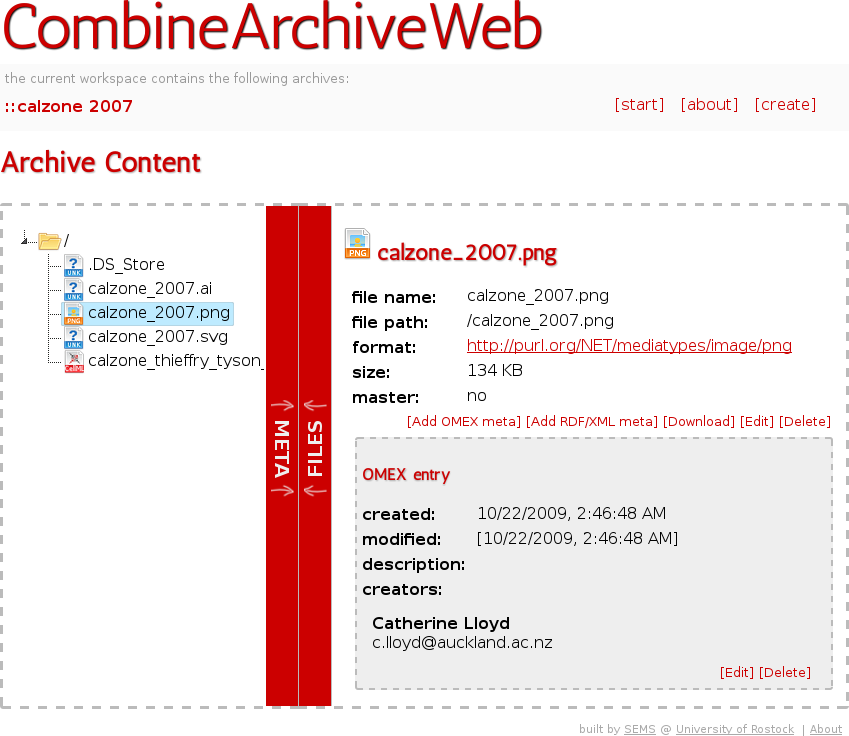
\includegraphics[width=.8\textwidth]{img/webcat-screenshot-combined.png}
\end{center}
\caption{\textbf{The CombineArchiveWeb application showing the archive as it was exported from M2CAT.} The files were cloned from the CellML model repository and immediately annotated with meta data. Thus, it is clear that I am not the creator of \textit{calzone\_2007.png}, instead it lists Catherine Lloyd as the creators and tells you when it was developed.}
\label{fig:screen:webcat}
\end{figure}

\subsection{Creating an initial COMBINE archive}

I created an initial version of the COMBINE archive using M2CAT~\cite{m2cat}.
The webinterface at \href{http://m2cat.sems.uni-rostock.de/}{m2cat.sems.uni-rostock.de} searches in a graph database to retrieve links to models published in open databases~\cite{masymos}.
The search for \texttt{Calzone} resulted in two matches, one of them representing the model in the CellML model repository.
In addition to searching in a graph database, M2CAT is also able to retrieve further the files that correspond to a simulation study.
For this it includes other sources, such as open model repositories, and bundles them in COMBINE archives using the library of the CombineArchive Toolkit~\cite{cat}.
Moreover, the web interface provides a link to conveniently explore the generated archive in the CombineArchiveWeb application~\cite{scharm2014}.

In case of the Calzone \emph{et.~al.} study, the files of the CellML model repository were cloned and aggregated in a new COMBINE archive.
Additionally, the resulting archive and its files were annotated with all the meta data available from the GIT project of the CellML model repositories.
Specifically, the archive was annotated with a description informing that it was generated by M2CAT.
The files that were cloned from the CellML model repository were annotated with creators, contributors, and modification times as available from the corresponding GIT project (\texttt{git log}), see Figure~\ref{fig:screen:webcat}.
Thus, the initial version of the COMBINE archive was obtained automatically.






\subsection{Extending the COMBINE archive}
\label{sec:extendingarchive}
As the initial version only contains the model encoded in CellML together with some figures (all files exclusively from the CellML model repository) I needed to extend the archive manually.
To organize the files I developed a file structure in the COMBINE archive containing the following directories:
\begin{itemize}
 \item \texttt{model/}: files that encode and visualise the biological system
 \item \texttt{experiment/}: files that encode the \textit{in silico} setup of the experiment
 \item \texttt{documentation/}: files that describe and document the model and/or experiment
 \item \texttt{result/}: files that result from running the experiment
\end{itemize}

Using the CombineArchiveWeb application it was very easy to get rid of the unrelated \texttt{.DS\_Store} file.
I also used the web interface to moved all other files into the model directory, as they all encoded the model.
Other directories are to be filled in the next sections.

\subsubsection{Retrieving Data and Information from other Services}
The first part of extending the archive dealt with a search for resources related to this study on the internet.
I was able to retrieve a journal publication and a model encoded in SBML.

\paragraph{The article} is usually the central object of a research study. As I said earlier, Calzone \emph{et.~al.} published their findings in Molecular Systems Biology. So I went to the corresponding website\footnote{\href{http://msb.embopress.org/content/3/1/131}{msb.embopress.org/content/3/1/131}} and downloaded the article and supplementary information.
As both describe the simulation experiment, I uploaded the files to the \texttt{documentation/} directory in the CombineArchiveWeb application.
The web interface decently added meta data listing me as the creator of the file, which, unfortunately, is in this case incorrect.
Thus, I modified the entries to attribute the real creators and to state when and where the files where downloaded.
Additionally, I added modification dates to the meta data of these files by copying them from the website of the article and the meta data of the PDF files.
The CombineArchiveWeb application provides a nice interface to modify the meta data without any necessity of touching or knowing about XML or RDF.
%knowledge about XML or RDF.
However, in the background it nevertheless created an RDF/XML tree to describe the article in a machine readable format, see section~\ref{sec:rdfmeta}.
This XML tree was then added ass a subtree to the meta data file of the archive.


\paragraph{The model} encoded in SBML format was already available from the Biomodels Database, so I went there to retrieve the file \texttt{BIOMD0000000144.xml}\footnote{\href{http://www.ebi.ac.uk/biomodels-main/download?mid=BIOMD0000000144}{www.ebi.ac.uk/biomodels-main/download?mid=BIOMD0000000144}} (SBML level 2 version 1).
The model file was then uploaded to the \texttt{model/} directory in the CombineArchiveWeb application and the meta data was modified to attribute the correct authors, curators, and contributors, according to the Biomodels Database website\footnote{\href{http://www.ebi.ac.uk/biomodels-main/BIOMD0000000144}{www.ebi.ac.uk/biomodels-main/BIOMD0000000144}} and as stated in the model document.


\subsubsection{Generating more Data}
The model files and the journal article are obviously not sufficient to reproduce the experiment's results.
However, I was not able to find any other information on the internet.
Thus, I generated more data myself.

\paragraph{The simulation description} is essential to run the experiment.
It defines the environment and the output of the \textit{in silico} execution.
Creating an initial simulation description was easy using the \sedml Web Tools\footnote{\href{http://bqfbergmann.dyndns.org/SED-ML_Web_Tools}{bqfbergmann.dyndns.org/SED-ML\_Web\_Tools}} (SWT).
I just needed to upload the model and to tick some boxes and the SWT created an initial \sedml script which runs a time course simulation on the model.
In the end it produces a graph for the concentration of every species and the value of every parameter and combines everything in a large table.
So I ended up with 66 plots and a huge table.
I compared the graphs with those shown in the paper and sensed a match.
That's a good start and I uploaded the \sedml \texttt{Calzone2007-simulation-all-figures.xml} script to the \texttt{experiment/} directory in the CombineArchiveWeb application.

To prove that the simulation setup reproduces the results described in \cite{Calzone2007} I developed another \sedml script \texttt{Calzone2007-simulation-figure-1B.xml} which generates Figure~1B of the publication.
This script was developed using the \textit{Edit Script} functionality of the SWT and is based on the initially generated script.
It produces both graphs shown on the right-hand side of Figure~1B in \texttt{documentation/Calzone2007.pdf}.
Finally, it was uploaded to the \texttt{experiment/} directory in the CombineArchiveWeb application.




\begin{figure}
\begin{center}
\subfigure[Figure~1B of the Publication]{
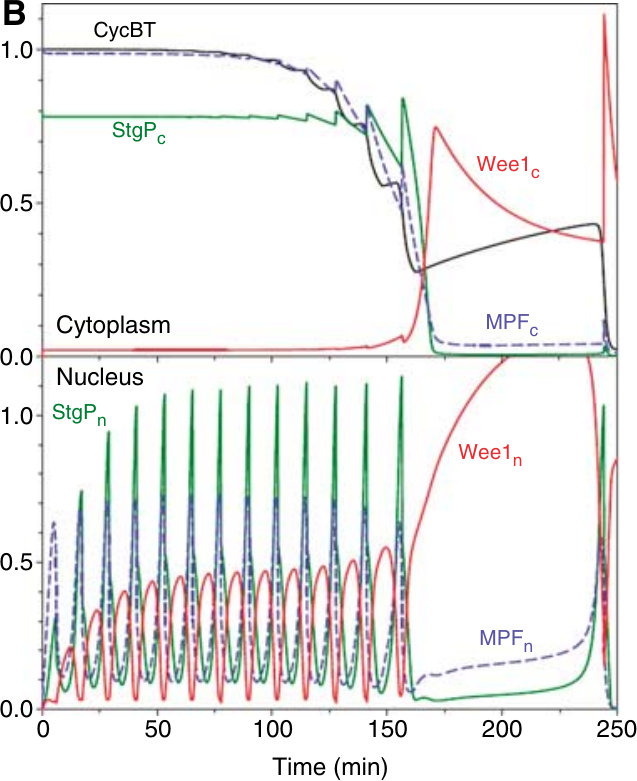
\includegraphics[width=.31\textwidth]{img/Figure1B-publication-trimmed.png}
\label{fig:sim:results:pub}
}
\subfigure[SED-ML Web Tools]{
\begin{minipage}[b]{.25\textwidth}
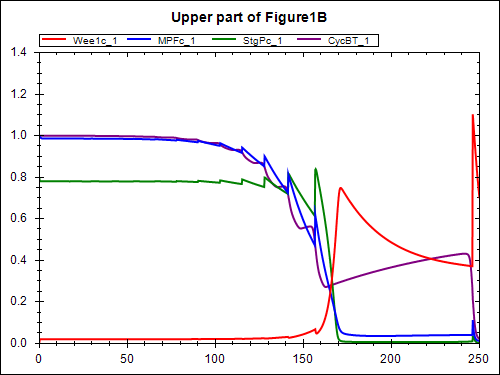
\includegraphics[width=\textwidth]{img/Fig1B-top-webtools.png}\\
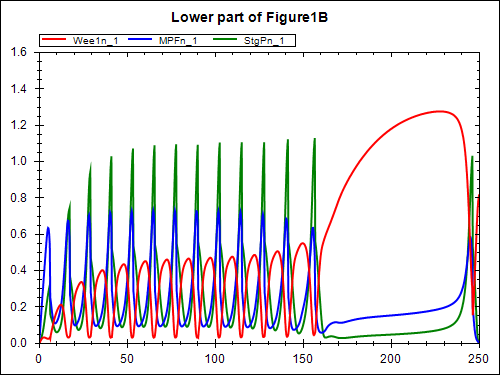
\includegraphics[width=\textwidth]{img/Fig1B-bottom-webtools.png}
\end{minipage}
\label{fig:sim:results:swt}
}
\subfigure[COPASI]{
\begin{minipage}[b]{.36\textwidth}
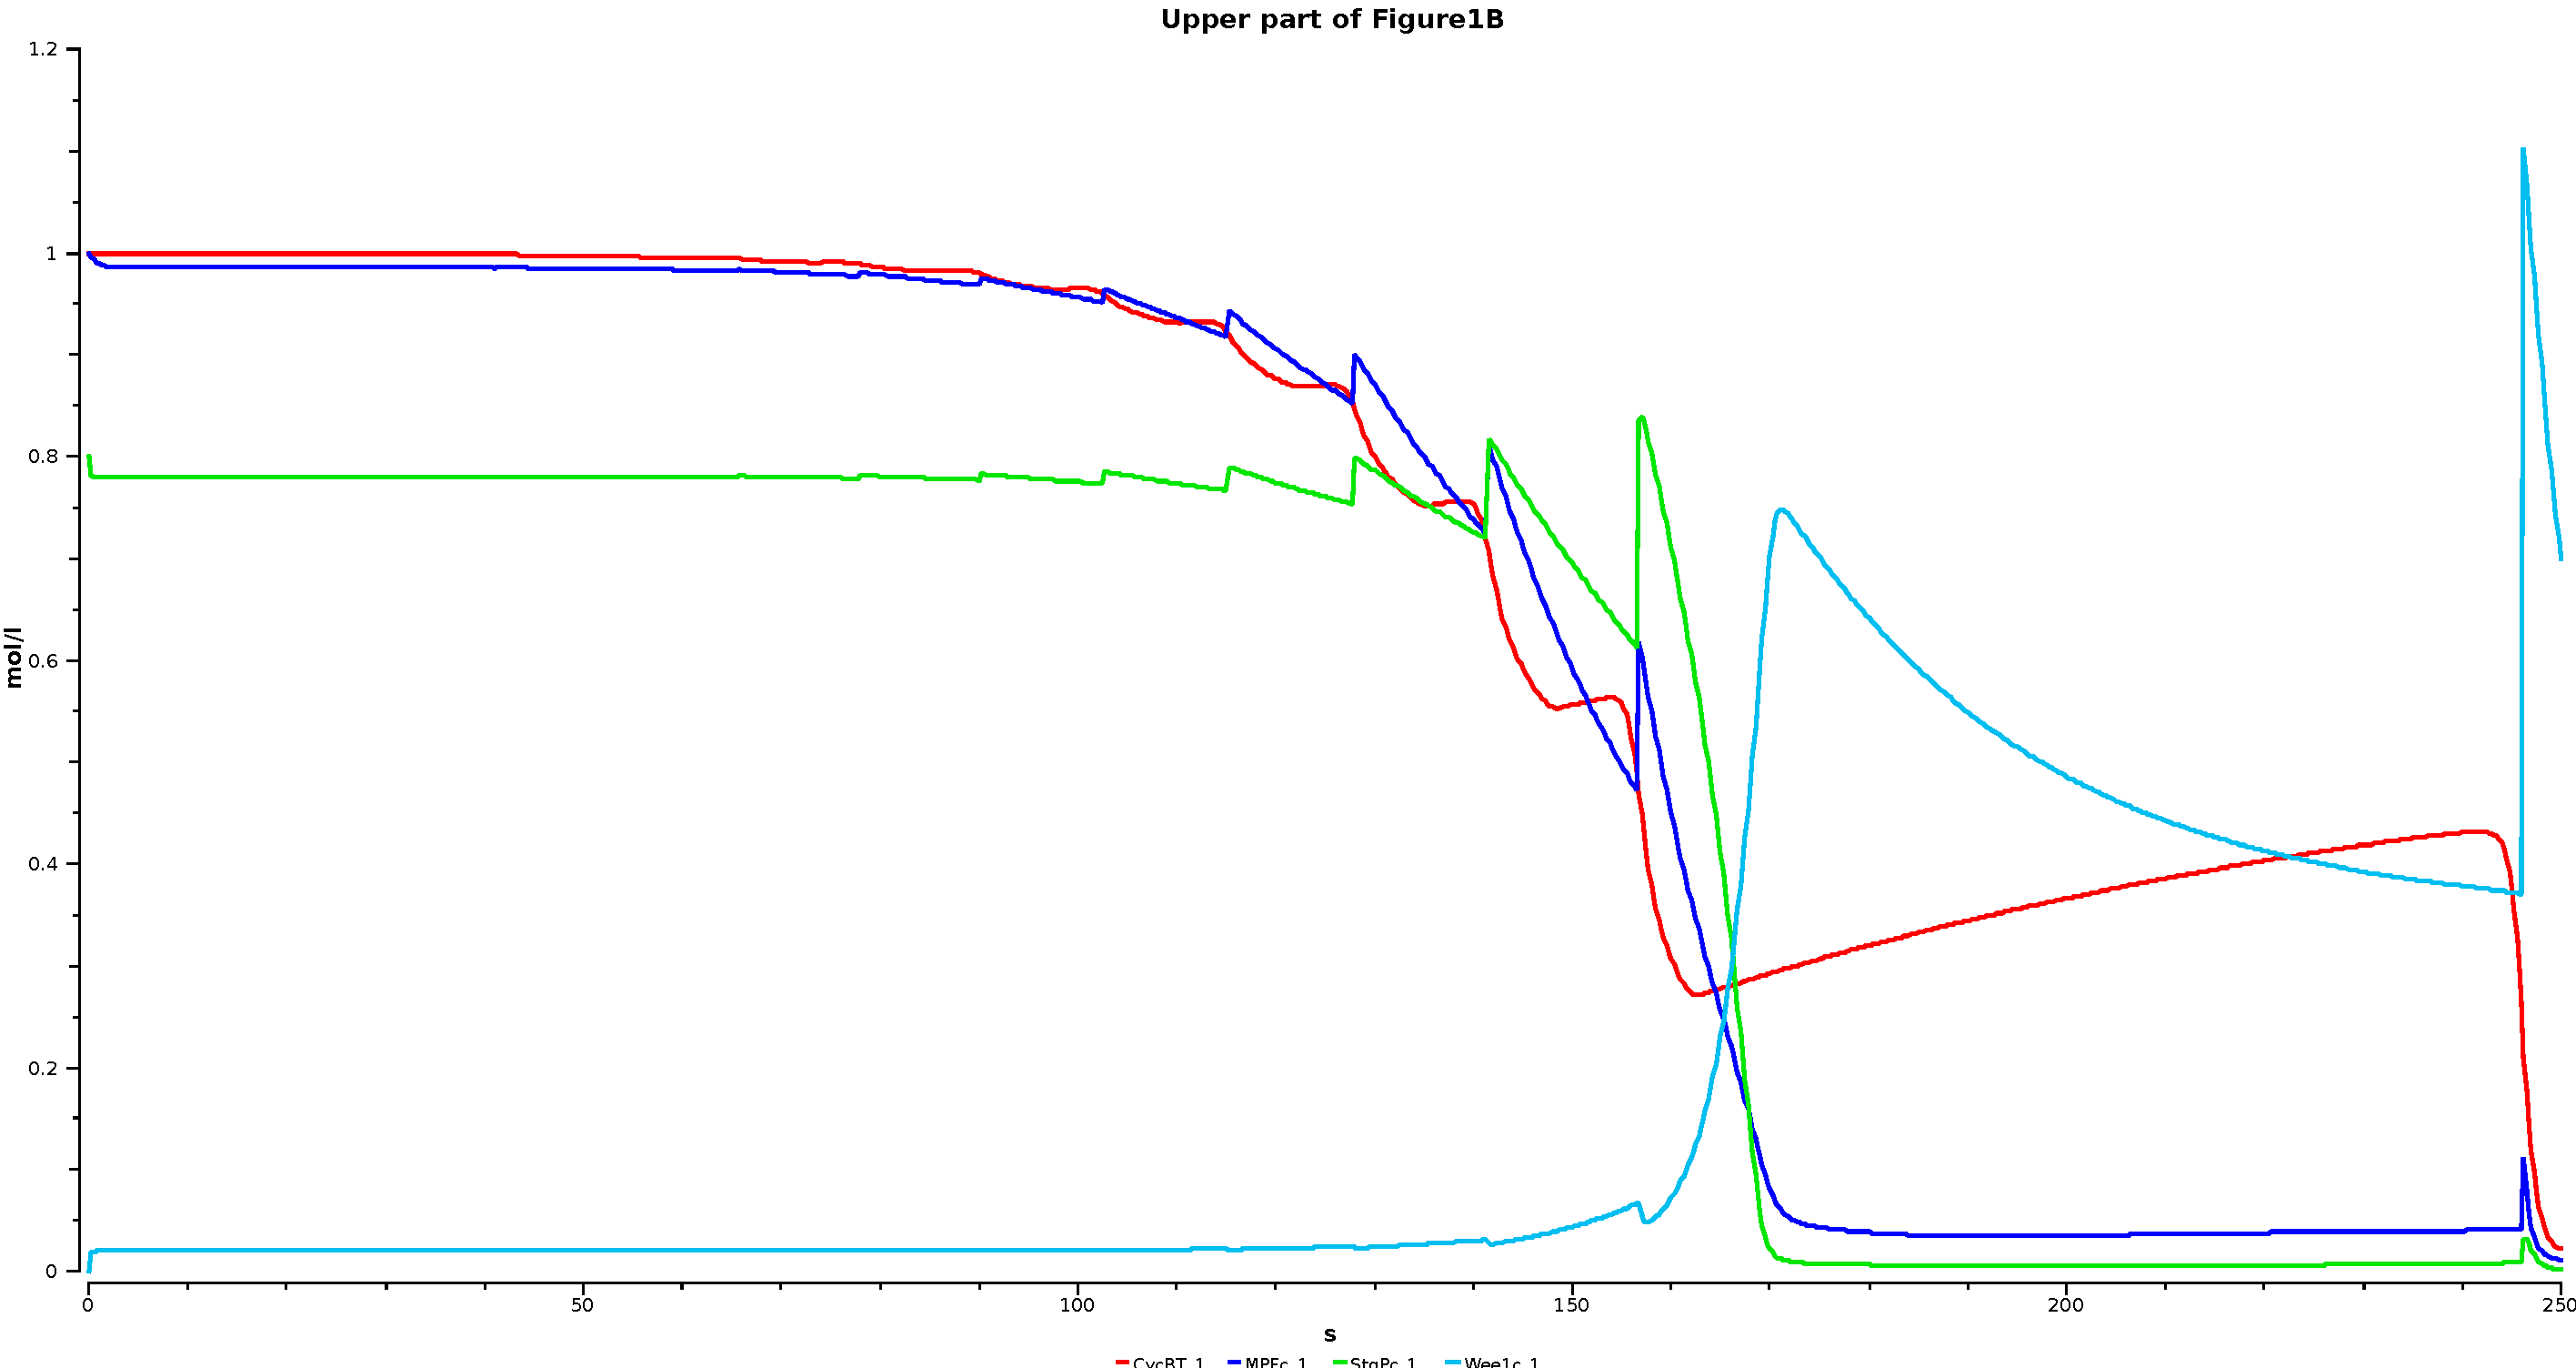
\includegraphics[width=\textwidth]{img/Fig1B-top-COPASI.pdf}\\
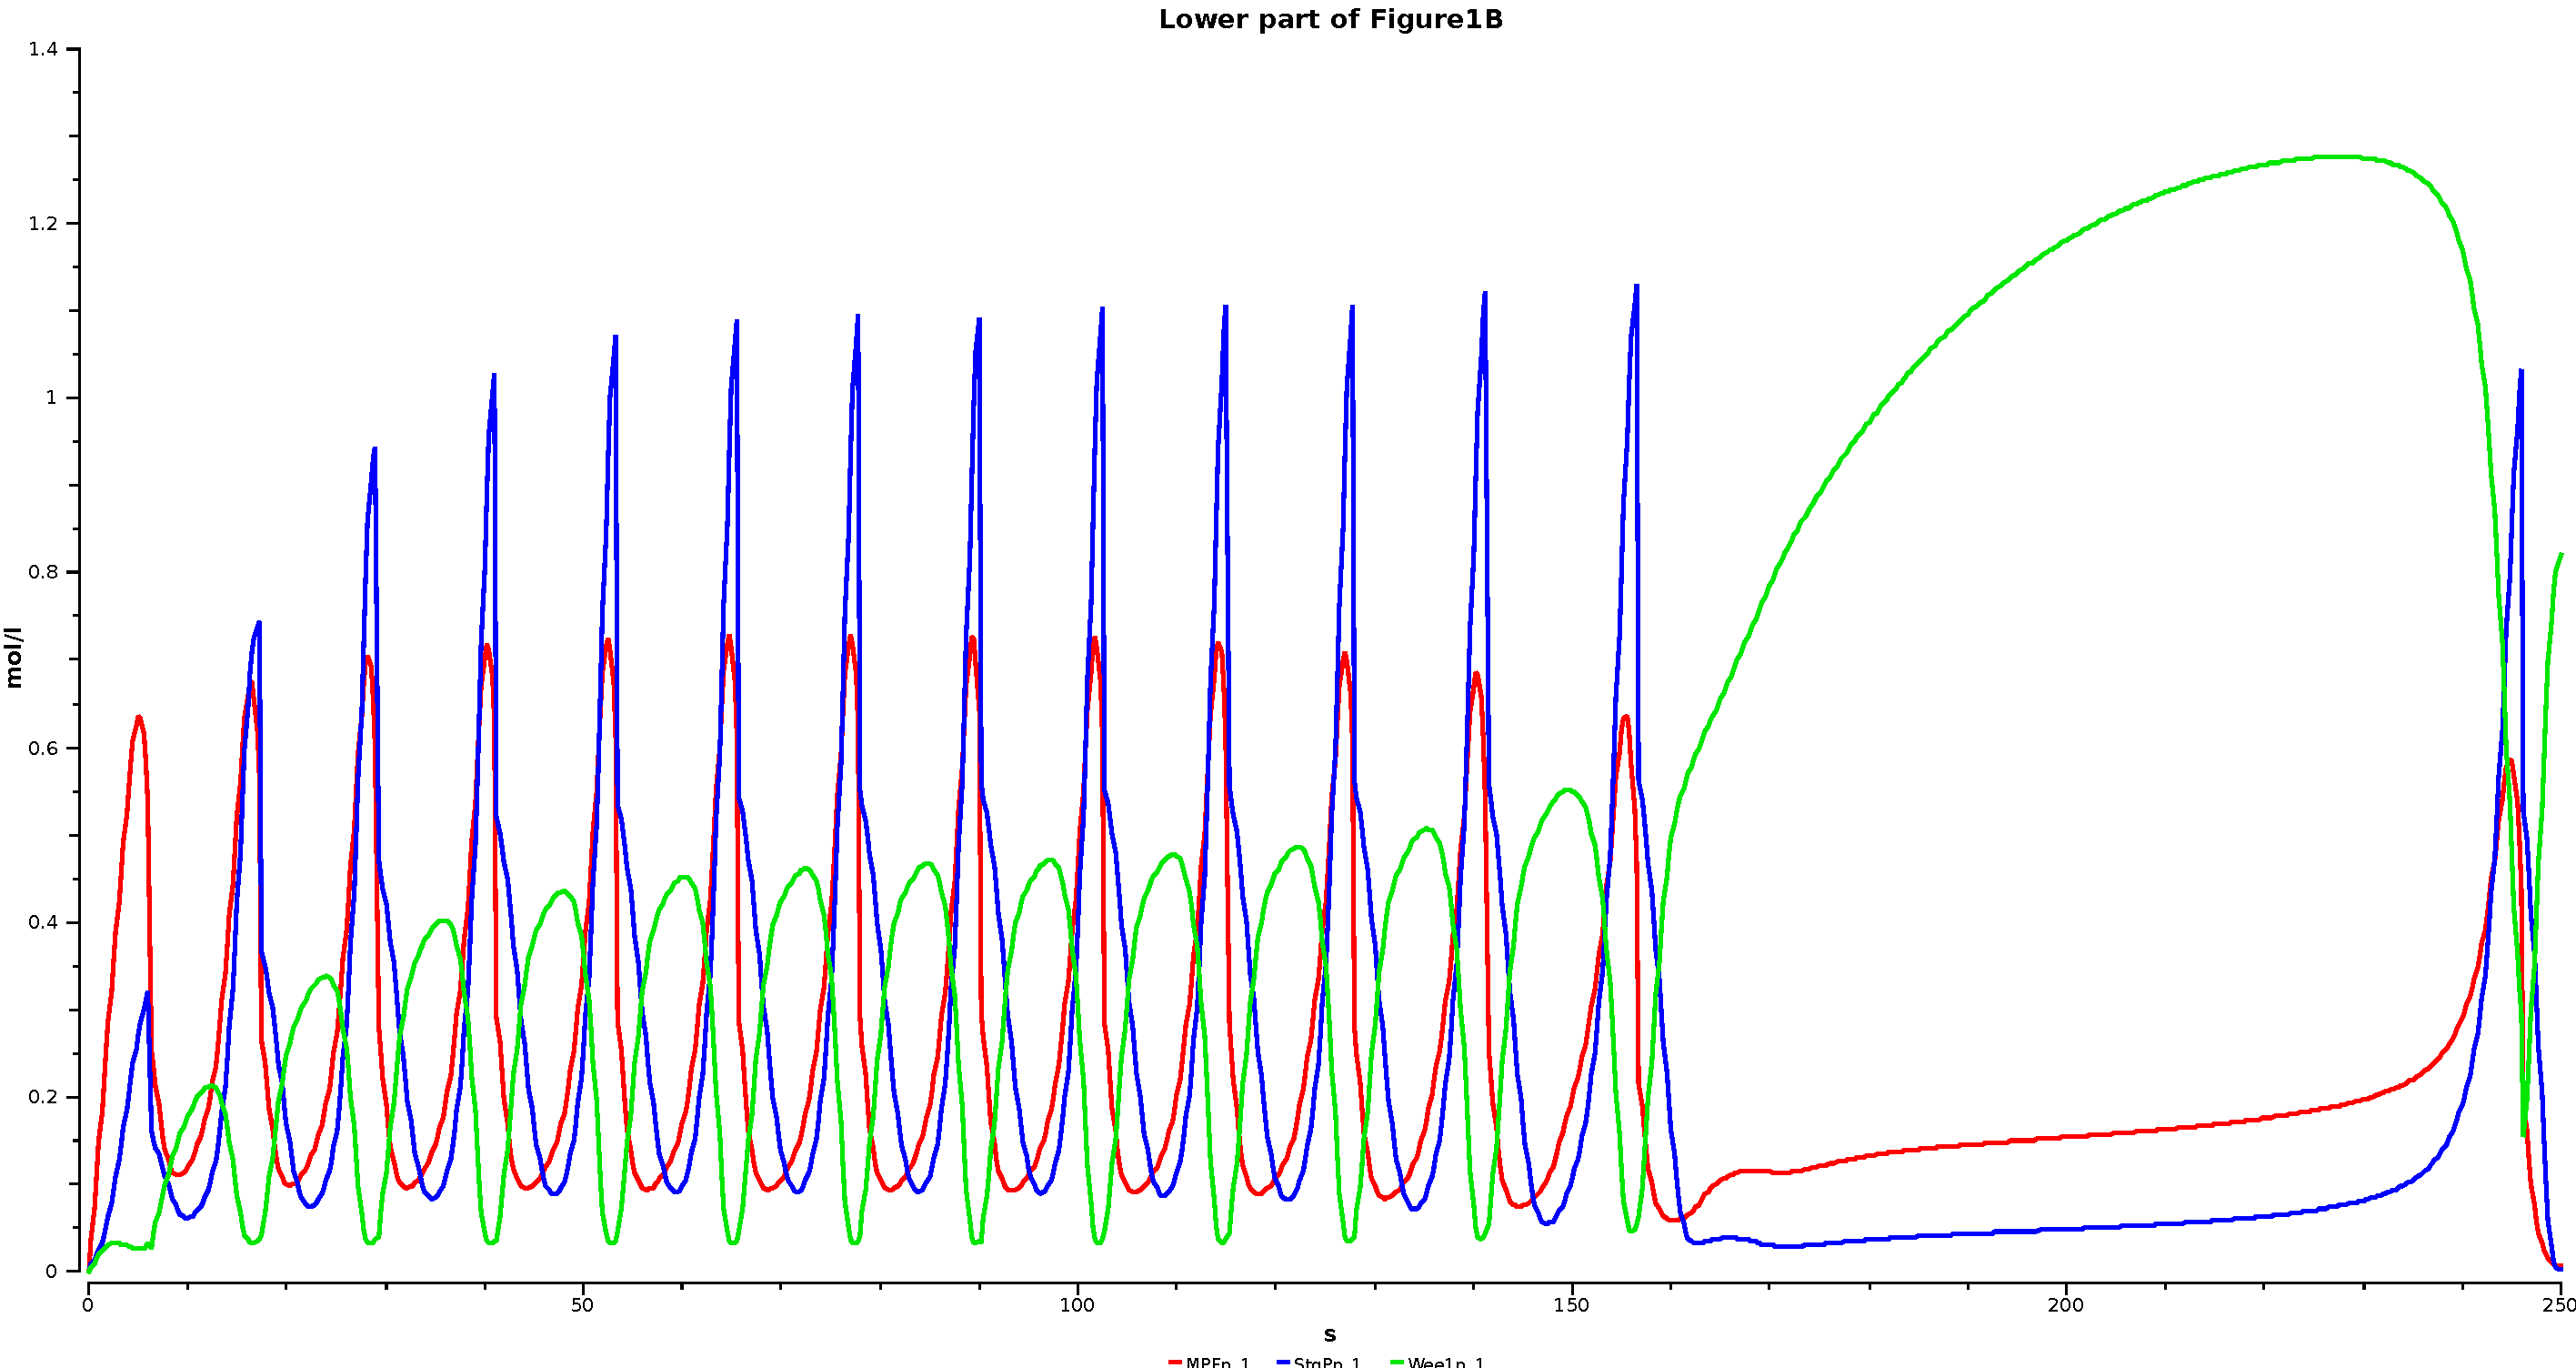
\includegraphics[width=\textwidth]{img/Fig1B-bottom-COPASI.pdf}
\end{minipage}
\label{fig:sim:results:COPASI}
}
\end{center}
\caption{\textbf{Comparison of simulation results.} The figure shows the simulation results included in the publication (\ref{fig:sim:results:pub}) with those results generated by the SWT (\ref{fig:sim:results:swt}) and COPASI (\ref{fig:sim:results:COPASI}) using the \sedml script \texttt{Calzone2007-simulation-figure-1B.xml}. It confirms that the results described in the publication could be reproduced.}
\label{fig:sim:results}
\end{figure}

\paragraph{The simulation results} show the effect of running the model under the environment defined in the simulation description.
To simulate the study I ran the experiment defined in \texttt{Calzone2007-simulation-figure-1B.xml} at the SWT and using the stand-alone software program COPASI~\cite{copasi}.
The plots generated by both tools prove that the developed \textit{in silico} experiment reproduce the figure shown in the publication, cmp. Figure~\ref{fig:sim:results}.
The SWT, see Figure~\ref{fig:sim:results:swt}, as well as COPASI, see Figure~\ref{fig:sim:results:COPASI}, were able to reproduce Figure~1B of the publication, see Figure~\ref{fig:sim:results:pub}.

The figures produced by the SWT and COPASI were uploaded to the \texttt{result/} directory in the CombineArchiveWeb application and meta data were added accordingly.



\begin{figure}
\begin{center}
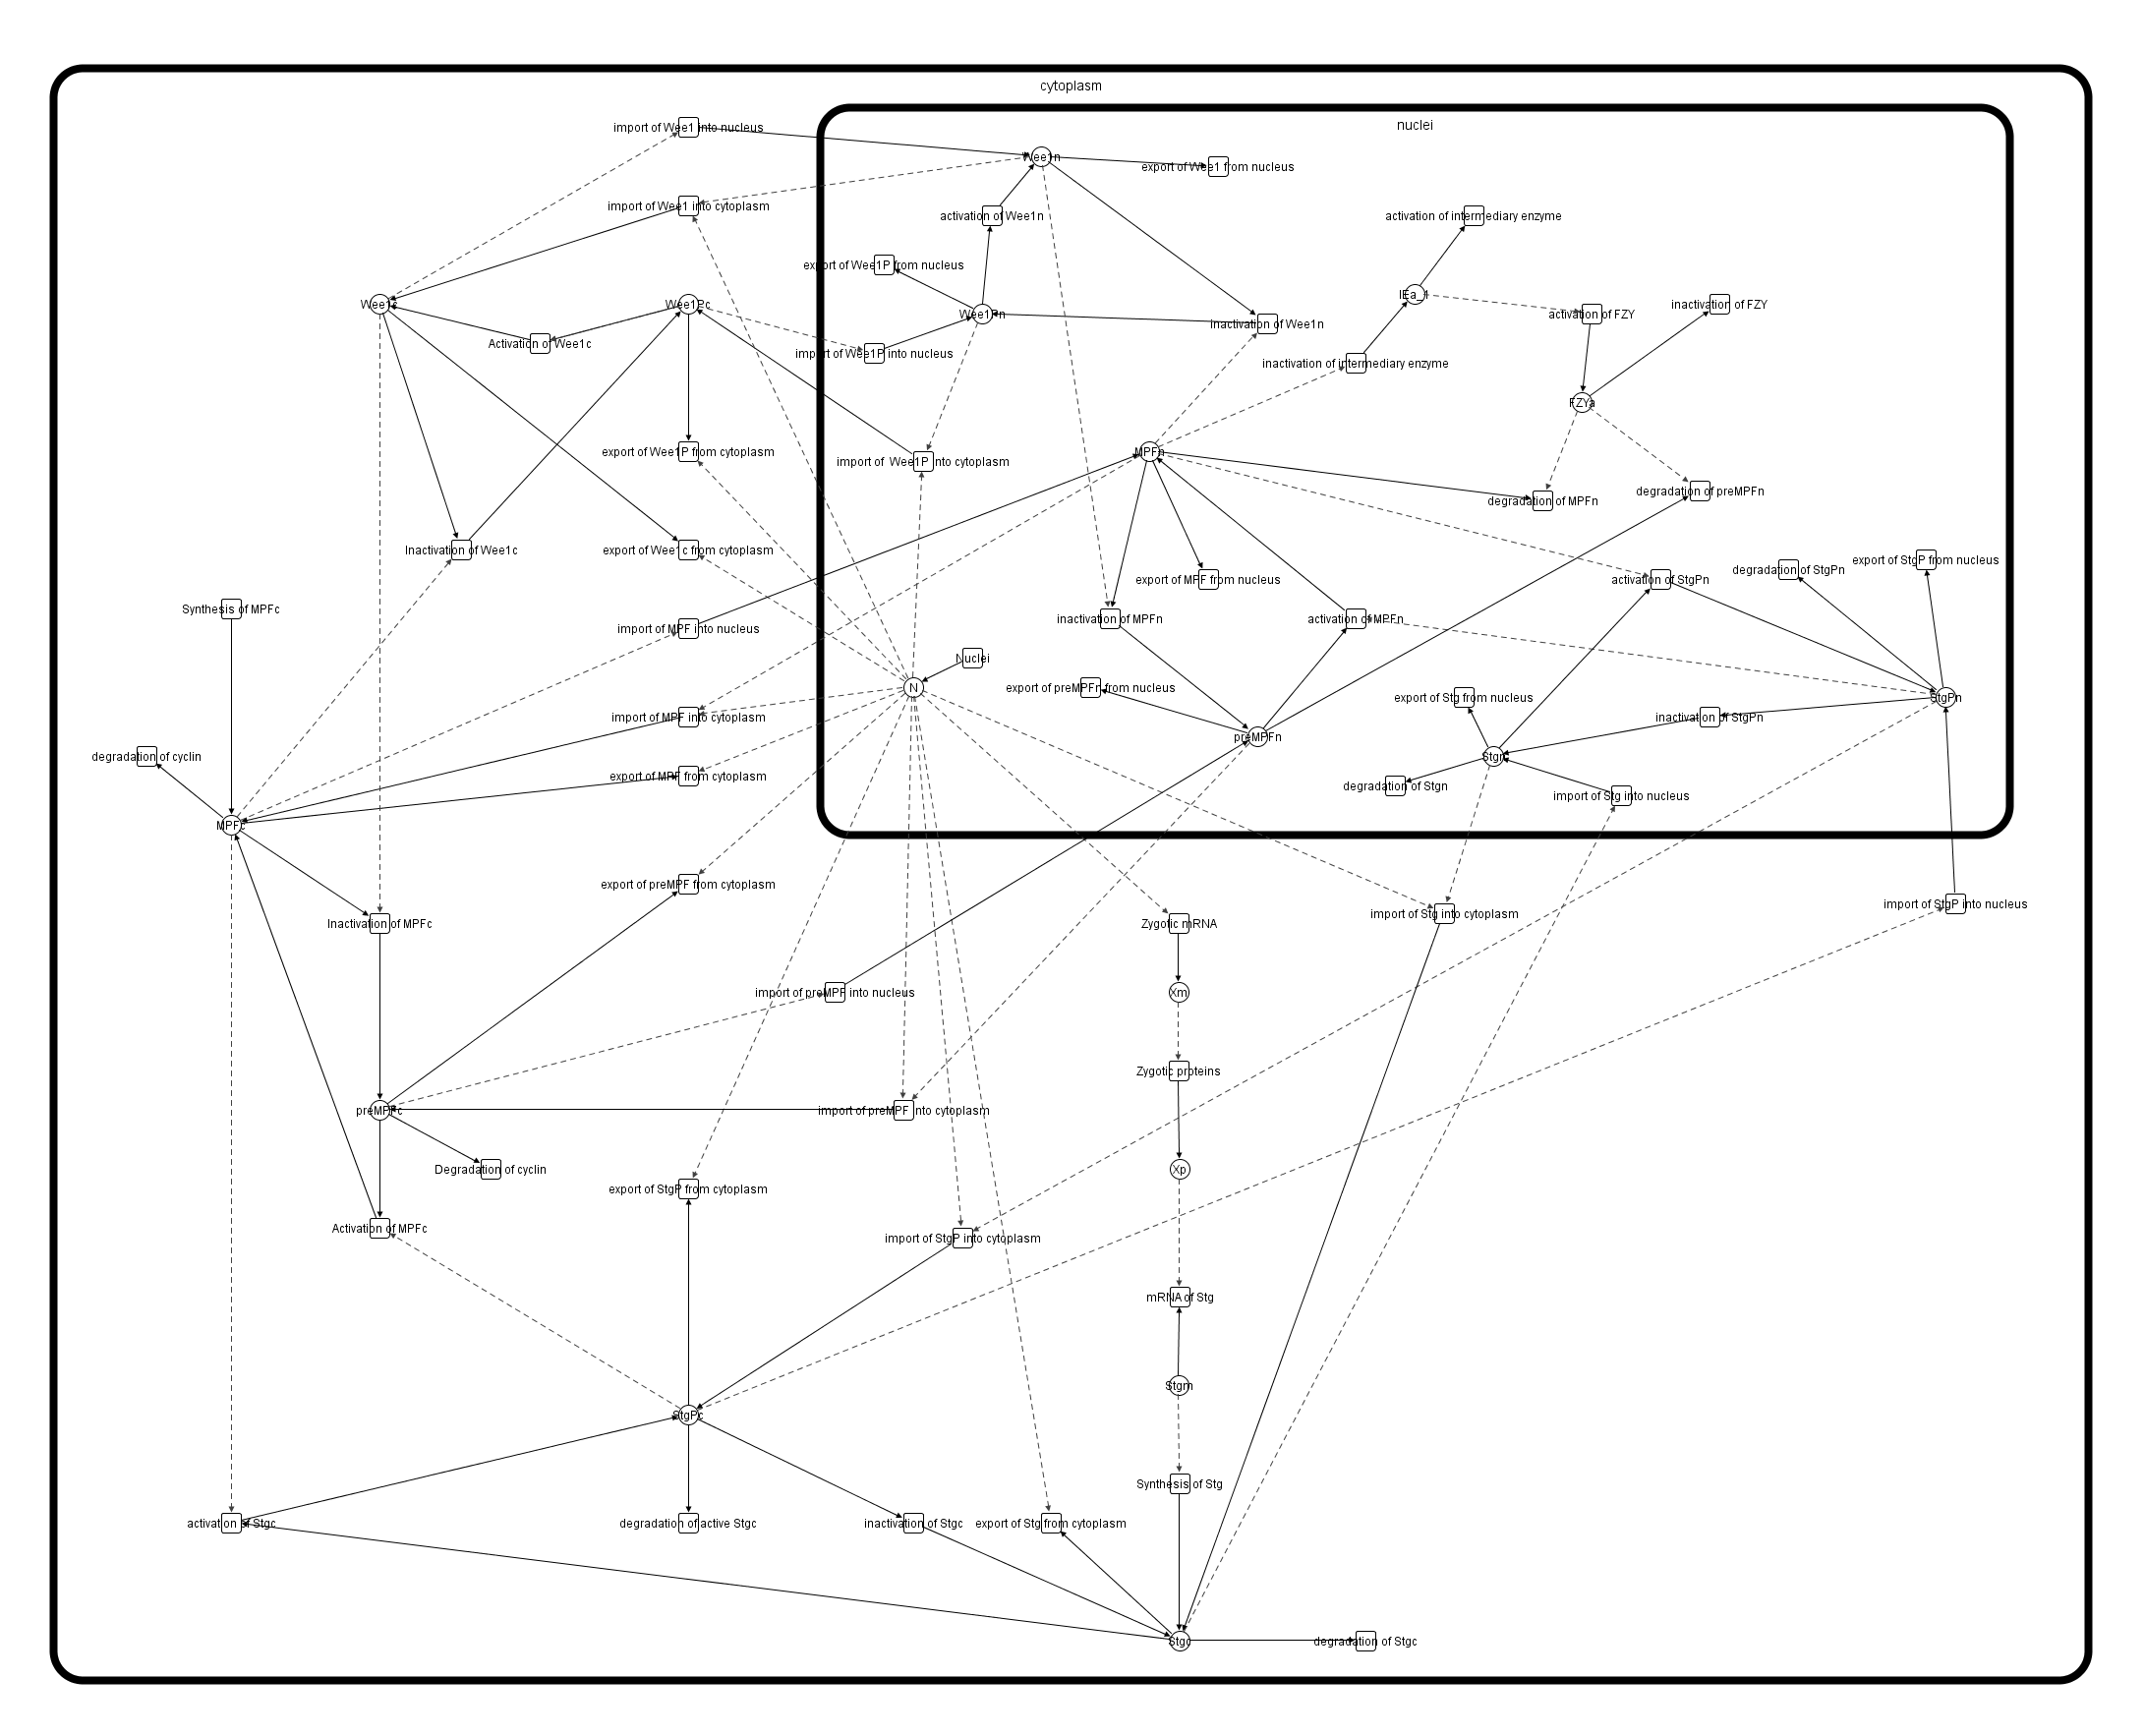
\includegraphics[width=.7\textwidth]{img/Calzone2007.png}
\end{center}
\caption{SBGN-compliant figure of the reaction network encoded in the model document.}
\label{fig:sbgngraph}
\end{figure}
\paragraph{The visualisation} displays the biological system.
There was a figure available from the CellML model repository, but it can also be encoded in a standard format.
I used SBGN-ED~\cite{sbgned} to load the SBML model, which immediately presented a layout of the reaction network encoded in the model.
After applying built-in graph layout algorithms from VANTED~\cite{vanted} and a bit of manual layouting I obtained the network, as shown in Figure~\ref{fig:sbgngraph}.
Due to an error in SBGN-ED, I was not able to export the figure in SBGN-ML layout, but uploaded it as GraphML~\cite{graphml}, GML\footnote{\href{http://www.fim.uni-passau.de/index.php?id=17297&L=1}{www.fim.uni-passau.de/index.php?id=17297\&L=1}}, PNG image, and PDF to the \texttt{model/sbgn} directory in the CombineArchiveWeb application.


























